\documentclass[10pt]{article}
\usepackage[margin=1.0cm,top=0.75cm,bottom=0.75cm,columnsep=0.5cm]{geometry}
\usepackage[utf8]{inputenc}
\usepackage[T1]{fontenc}
\usepackage{lmodern}
\usepackage{microtype}
\usepackage{multicol}
\usepackage{booktabs}
\usepackage{xcolor}
\usepackage{hyperref}
\usepackage{tikz}
\usetikzlibrary{positioning,arrows.meta,calc}

\definecolor{ucblue}{RGB}{0,51,102}
\definecolor{toolgray}{RGB}{110,110,110}
\hypersetup{colorlinks=true,urlcolor=ucblue,linkcolor=ucblue}
\setlength{\parindent}{0pt}
\setlength{\parskip}{2pt}
\pagestyle{empty}
\newcommand{\head}[1]{\textbf{\color{ucblue}#1}\hspace{0.4em}}
\newcommand{\pendiente}[1]{\textcolor{red}{[PENDIENTE: #1]}}
\newcommand{\VideoURL}{\href{https://drive.google.com/file/d/1I9KuGPZe99HninfvLdC2E1XQjTf00EQZ/view?usp=sharing}{Google Drive}}

\begin{document}

\begin{center}
{\Large\bfseries\color{ucblue} SQL4Business: Deliverable 3 --- sistema de agentes}\\[2pt]
{\small Generative Artificial Intelligence (580694), Universidad de Concepci\'on}\\[1pt]
{\small Aredhel Jim\'enez, Bryan Riquelme, Guido Salazar, Vicente So\~nez}\\[1pt]
{\small C\'odigo: \href{https://github.com/aredhel-jmze/Asistente-SQL-4-Business}{github.com/aredhel-jmze/Asistente-SQL-4-Business}
\quad$\vert$\quad Video: \VideoURL}
\end{center}

\vspace{-4pt}
\begin{center}
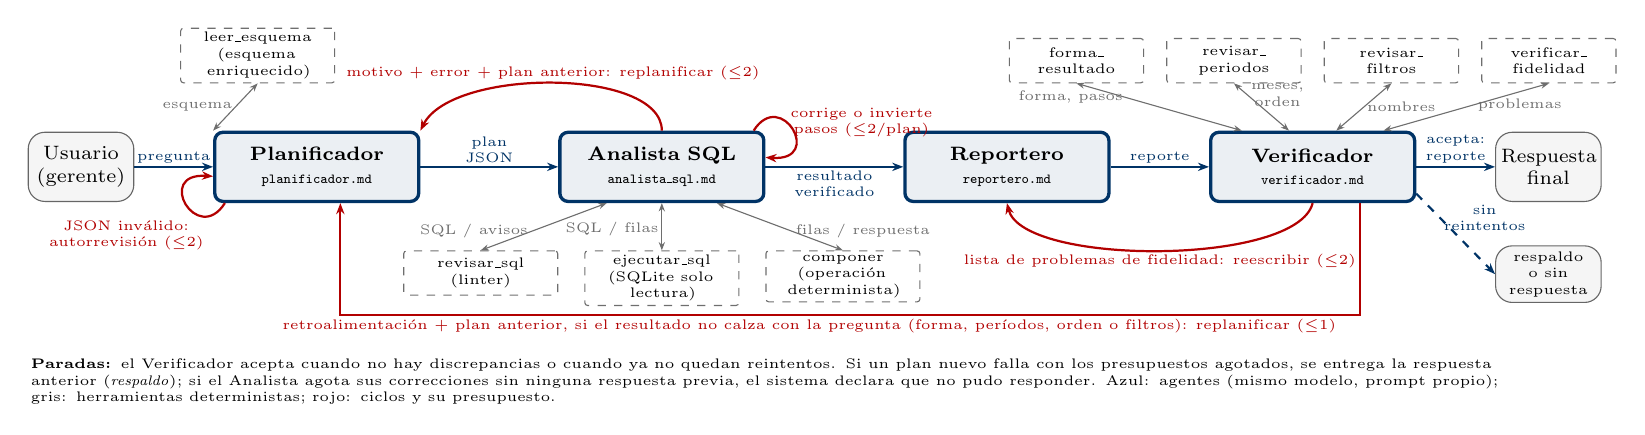
\begin{tikzpicture}[
  font=\scriptsize,
  agent/.style={draw=ucblue, fill=ucblue!8, very thick, rounded corners=3pt, align=center, minimum height=2.5em, text width=2.45cm, inner sep=2pt},
  tool/.style={draw=toolgray, dashed, rounded corners=1pt, align=center, font=\tiny, inner sep=1.5pt, minimum height=1.6em, text width=1.85cm},
  vtool/.style={tool, text width=1.6cm},
  ext/.style={draw=black!60, fill=black!4, rounded corners=6pt, align=center, minimum height=2.5em, text width=1.2cm, inner sep=2pt},
  flow/.style={-{Stealth[length=4pt]}, thick, ucblue},
  back/.style={-{Stealth[length=4pt]}, thick, red!70!black},
  use/.style={{Stealth[length=3pt]}-{Stealth[length=3pt]}, toolgray},
  lab/.style={font=\tiny, inner sep=1pt, align=center}]
  \node[ext] (u) {Usuario\\(gerente)};
  \node[agent, right=1.0cm of u] (p) {\textbf{Planificador}\\{\tiny\ttfamily planificador.md}};
  \node[agent, right=1.75cm of p] (a) {\textbf{Analista SQL}\\{\tiny\ttfamily analista\_sql.md}};
  \node[agent, right=1.75cm of a] (r) {\textbf{Reportero}\\{\tiny\ttfamily reportero.md}};
  \node[agent, right=1.25cm of r] (v) {\textbf{Verificador}\\{\tiny\ttfamily verificador.md}};
  \node[ext, right=1.0cm of v] (o) {Respuesta\\final};
  \node[ext, below=0.55cm of o, text width=1.2cm, font=\tiny, minimum height=2em] (s) {respaldo\\o sin\\respuesta};

  \node[tool, above=0.6cm of p, xshift=-0.75cm] (t1) {leer\_esquema\\(esquema enriquecido)};
  \node[tool, below=0.6cm of a, xshift=-2.3cm] (t2) {revisar\_sql\\(linter)};
  \node[tool, below=0.6cm of a] (t3) {ejecutar\_sql\\(SQLite solo lectura)};
  \node[tool, below=0.6cm of a, xshift=2.3cm] (t4) {componer\\(operación determinista)};
  \node[vtool, above=0.6cm of v, xshift=-3.0cm] (t5) {forma\_\\resultado};
  \node[vtool, above=0.6cm of v, xshift=-1.0cm] (t6) {revisar\_\\periodos};
  \node[vtool, above=0.6cm of v, xshift=1.0cm] (t8) {revisar\_\\filtros};
  \node[vtool, above=0.6cm of v, xshift=3.0cm] (t7) {verificar\_\\fidelidad};

  \draw[flow] (u) -- node[lab, above] {pregunta} (p);
  \draw[flow] (p) -- node[lab, above] {plan\\JSON} (a);
  \draw[flow] (a) -- node[lab, below] {resultado\\verificado} (r);
  \draw[flow] (r) -- node[lab, above] {reporte} (v);
  \draw[flow] (v) -- node[lab, above] {acepta:\\reporte} (o);
  \draw[flow, dashed] ($(v.south east)+(0,0.12)$) -- node[lab, right, pos=0.3, text=ucblue] {sin\\reintentos} (s.west);

  \draw[use] (t1.south) -- node[lab, left] {esquema} (p.north west |- p.north) ;
  \draw[use] (t2.north) -- node[lab, left, pos=0.4] {SQL / avisos} ($(a.south)+(-0.7,0)$);
  \draw[use] (t3.north) -- node[lab, left, pos=0.45] {SQL / filas} (a.south);
  \draw[use] (t4.north) -- node[lab, right, pos=0.4] {filas / respuesta} ($(a.south)+(0.7,0)$);
  \draw[use] (t5.south) -- node[lab, left, pos=0.3] {forma, pasos} ($(v.north)+(-0.9,0)$);
  \draw[use] (t6.south) -- node[lab, right, pos=0.25] {meses,\\orden} ($(v.north)+(-0.3,0)$);
  \draw[use] (t8.south) -- node[lab, right, pos=0.5] {nombres} ($(v.north)+(0.3,0)$);
  \draw[use] (t7.south) -- node[lab, right, pos=0.45] {problemas} ($(v.north)+(0.9,0)$);

  \draw[back] ($(p.south west)+(0.15,0)$) .. controls +(-0.35,-0.55) and +(-0.75,0.05) .. node[lab, below left, pos=0.2] {JSON inválido:\\autorrevisión ($\leq$2)} ($(p.west)+(0,-0.12)$);
  \draw[back] ($(a.north east)+(-0.15,0)$) .. controls +(0.35,0.55) and +(0.75,-0.05) .. node[lab, right, pos=0.4] {corrige o invierte\\pasos ($\leq$2/plan)} ($(a.east)+(0,0.12)$);
  \draw[back] (a.north) .. controls +(0,0.8) and +(0.4,0.8) .. node[lab, above] {motivo + error + plan anterior: replanificar ($\leq$2)} (p.north east);
  \draw[back] (v.south) .. controls +(-0.2,-0.8) and +(0.2,-0.8) .. node[lab, below] {lista de problemas de fidelidad: reescribir ($\leq$2)} (r.south);
  \draw[back] ($(v.south)+(0.6,0)$) -- ++(0,-1.42) -| node[lab, pos=0.27, below] {retroalimentación + plan anterior, si el resultado no calza con la pregunta (forma, períodos, orden o filtros): replanificar ($\leq$1)} ($(p.south)+(0.3,0)$);
  \node[lab, text width=18.6cm, align=left, anchor=north west, font=\tiny] at ($(u.south west)+(0,-1.95)$)
    {\textbf{Paradas:} el Verificador acepta cuando no hay discrepancias o cuando ya no quedan reintentos. Si un plan nuevo falla con los presupuestos agotados, se entrega la respuesta anterior (\textit{respaldo}); si el Analista agota sus correcciones sin ninguna respuesta previa, el sistema declara que no pudo responder. Azul: agentes (mismo modelo, prompt propio); gris: herramientas deterministas; rojo: ciclos y su presupuesto.};
\end{tikzpicture}
\end{center}
\vspace{-8pt}

\begin{multicols}{2}
\small

\head{Tarea, continuidad y modelo.} La misma tarea, falla y criterio de salida correcta de los
entregables anteriores. Las piezas deterministas del D2 pasan a ser herramientas de los
agentes y el código del D2 no cambia. Los cuatro agentes usan el mismo modelo, \texttt{Qwen/Qwen2.5-Coder-3B-Instruct} (revisión \texttt{488639f}, NF4 de
4 bits, decodificación greedy, Colab T4), con un prompt propio por agente en \texttt{prompts/}.

\head{Agentes, decisiones y división del trabajo.} El \textbf{Planificador} elige los pasos SQL y
la operación de composición, que define qué calculará el Analista; si su JSON no es válido, lo revisa.
El \textbf{Analista SQL} ejecuta el plan con sus herramientas y solo llama al modelo cuando una
falla: el modelo decide corregir un paso, invertir dos o devolver el plan. El \textbf{Reportero}
decide qué cifras citar y, si lo rechazan, reescribe. En el \textbf{Verificador}, el modelo lee solo
la pregunta y declara qué pide y qué períodos nombra; una regla compara eso con sus herramientas y
decide devolver el plan, devolver el reporte o aceptar. Son cuatro competencias distintas (entender,
ejecutar, redactar, juzgar) y quien juzga no produce el trabajo.

\head{Técnicas de prompting} (Schulhoff et al., 2024; todos usan \textit{role prompting} y salida
estructurada). \textit{Planificador:} (1) \textbf{few-shot}, tres ejemplos fuera de la evaluación,
contra listados en vez del primero y \texttt{strftime('\%Q')}; (2) \textbf{descomposición}
(\textit{plan-and-solve}): lo que pide la respuesta y los períodos antes del SQL, contra una sola
consulta para preguntas de varios valores. \textit{Analista:} (3) \textbf{autocorrección guiada por
herramientas} (\textit{self-debugging}), contra errores de fechas y sintaxis (q09, q10).
\textit{Verificador:} (4) \textbf{lista de chequeo} (\textit{self-verification}) contrastada con
herramientas, contra resultados válidos que no responden la pregunta (q03, q11, q09-p, q14-p).
\textit{Reportero:} (5) \textbf{self-refine}, contra cifras no respaldadas (q13). Cada técnica se
apaga por separado.

\head{Evaluación.} 15 preguntas del D1 (10 puntuales, 5 combinadas; in-sample) y 12 paráfrasis
(5/7). Mismo criterio para todos: \textit{sql} (D1), \textit{answer} (respuesta correcta),
\textit{e2e} (y reporte fiel).

\head{Resultados.} El sistema (v2) responde con reporte fiel 12/15 oficiales y 11/12
paráfrasis, frente a 10/15 y 10/12 del D2; en combinadas, 3/5 y 6/7 frente a 2/5 y 5/7. Frente
al D2 se ganan 6 preguntas y se pierden 3 (q04, q12, q11-p); el detalle por pregunta está en el
README. En la
ablación, sin few-shot se pierden 2 y 1 preguntas; sin el Verificador, 1 y 1 (corrigió q11 y
q08-p); sin refinamiento, un reporte (q10-p). La descomposición suma 3 combinadas externas pero
cuesta una puntual oficial (q04). La autocorrección no se puede medir aquí: el Analista consultó
al modelo 2 veces en 27 preguntas, porque casi no hubo errores de SQL. Con 27 preguntas, una
diferencia de 1 o 2 es una tendencia. Costo: 3,6 llamadas y 33\,s por pregunta (D2: 2,1 y 15\,s).

\head{Caso de falla: q12.} El Planificador ordena los pasos como los nombra la pregunta (agosto
antes que marzo) y el código calcula una caída de 37,14\,\% en vez de un alza de 59,08\,\%. El
Verificador lo detecta (control de orden de \texttt{revisar\_periodos}) y lo devuelve con el motivo exacto, pero el Planificador, con decodificación
greedy y un sesgo fuerte por el orden de la pregunta, repite el mismo plan; agotado el reintento, el
sistema acepta. En q04 (falta el filtro \textit{Alimentos}) pasa lo mismo: detectar no basta si el
agente que corrige ignora la retroalimentación. Trazas: \texttt{trazas/official\_q12.json} y
\texttt{demo/q12.json} (en \texttt{results/deliverable3/}, la segunda con el control de orden registrado).

\head{Límites.} El Verificador depende de que el modelo clasifique bien la pregunta (en q10 la
lee como lista). Conjuntos chicos y sintéticos.

\head{Desviaciones declaradas.} Linter \texttt{revisar\_sql} y una regla de fidelidad compartida con
el D2 que no altera sus veredictos. Tras v1, el ejemplo de cambio porcentual del Reportero solo
aparece si aplica, el Verificador suma \texttt{revisar\_filtros}, orden y pasos descartados, y el
Analista puede invertir pasos; por eso las paráfrasis ya no son estrictamente externas.

\head{Reproducción.} \texttt{notebooks/deliverable3\_demo.ipynb} (Colab T4): demo
(\texttt{run\_agents.py}) y evaluación (\texttt{evaluate\_d3.py}), con trazas en \texttt{results/}.
\end{multicols}

\vspace{-6pt}
\begin{center}
\footnotesize
\begin{tabular}{@{}lccccccc@{}}
\toprule
& \multicolumn{3}{c}{\textbf{Set oficial (15)}} & \multicolumn{3}{c}{\textbf{Paráfrasis (12)}} & \\
\cmidrule(lr){2-4}\cmidrule(lr){5-7}
\textbf{Configuración} & sql & answer & e2e & sql & answer & e2e & \textbf{Llamadas} \\
\midrule
Prompt directo (baseline D1) & 7/15 & 8/15 & -- & 3/12 & 5/12 & -- & 1.0 \\
Solución D2 (pipeline) & 11/15 & 11/15 & 10/15 & 8/12 & 10/12 & 10/12 & 2.1 \\
\addlinespace
Agentes v1 (primera corrida) & 11/15 & 11/15 & 9/15 & 9/12 & 11/12 & 9/12 & 3.8 \\
Sistema de agentes v2 (D3) & 11/15 & 12/15 & 12/15 & 9/12 & 11/12 & 11/12 & 3.6 \\
\addlinespace
\quad sin ejemplos (few-shot) & 9/15 & 10/15 & 10/15 & 8/12 & 10/12 & 10/12 & 3.4 \\
\quad sin descomposición explícita & 10/15 & 13/15 & 13/15 & 6/12 & 8/12 & 8/12 & 3.3 \\
\quad sin autocorrección del Analista & 11/15 & 12/15 & 12/15 & 9/12 & 11/12 & 11/12 & 3.5 \\
\quad sin verificación crítica & 11/15 & 11/15 & 11/15 & 8/12 & 10/12 & 10/12 & 2.1 \\
\quad sin refinamiento del reporte & 11/15 & 12/15 & 12/15 & 9/12 & 11/12 & 10/12 & 3.6 \\
\bottomrule
\end{tabular}

\end{center}

\end{document}
